\documentclass{article}
\usepackage{amsmath}
\usepackage{changepage}
\usepackage{float}
\usepackage{amsmath}
\usepackage{tikz}
\usepackage{graphicx}
\usepackage{color}
\usepackage{listings}
\usepackage{color}
\usepackage{algpseudocode}
\definecolor{dkgreen}{rgb}{0,0.6,0}
\definecolor{gray}{rgb}{0.5,0.5,0.5}
\definecolor{mauve}{rgb}{0.58,0,0.82}
\usetikzlibrary{arrows}

\lstset{frame=tb,
  language=Java,
  aboveskip=3mm,
  belowskip=3mm,
  showstringspaces=false,
  columns=flexible,
  basicstyle={\small\ttfamily},
  numbers=none,
  numberstyle=\tiny\color{gray},
  keywordstyle=\color{blue},
  commentstyle=\color{dkgreen},
  stringstyle=\color{mauve},
  breaklines=true,
  breakatwhitespace=true,
  tabsize=3
}

\long\def\/*#1*/{}

\tikzset{
  treenode/.style = {align=center, inner sep=0pt, text centered,
    font=\sffamily},
  1/.style = {treenode, circle, white, font=\sffamily\bfseries, draw=black,
    fill=black, text width=1.5em},% arbre rouge noir, noeud noir
  2/.style = {treenode, circle, white, draw=black, 
    text width=1.5em, very thick},% arbre rouge noir, noeud rouge
  %3/.style = {treenode, circle, white, draw=black,
    %minimum width=0.5em, minimum height=0.5em}% arbre rouge noir, nil
}

\begin{document}
\begin{center}
Andreas Bach Landgrebe \\
Computer Science 250: Analysis of Algorithms \\
February 25, 2015 \\
Laboratory Assignment 5 - Exhaustive Search – Eight Queens \\
\end{center}
\newpage
\noindent
Part 1: Implementing Basic Eight Queens \& \\ Part 2: Implementing Advanced Eight Queens \\
\begin{center}
Source Code
\end{center}
\begin{lstlisting}
import java.util.Scanner;


public class eightQueens {

	static int QueensFive[] = new int[5];

	static int QueensEight[] = new int[8];

	static int QueensEleven[] = new int[11];

	static int solutions =0;
	
	public static boolean isGoodEight(int row, int col) {
		int colLeft=col-1;
		int colRight=col+1;
		for (int i=row-1; i>=0; i--) {
			if (QueensEight[i]==colLeft--) return false;
			if (QueensEight[i]==col) return false;
			if (QueensEight[i]==colRight++) return false;
		} //for
		return true;
	} //isGoodEight

	public static boolean isGoodFive(int row, int col) {
		int colLeft=col-1;
		int colRight=col+1;
		for (int i=row-1; i>=0; i--) {
			if (QueensFive[i]==colLeft--) return false;
			if (QueensFive[i]==col) return false;
			if (QueensFive[i]==colRight++) return false;
		} //for
		return true;
	} //isGoodFive

	public static boolean isGoodEleven(int row, int col) {
		int colLeft=col-1;
		int colRight=col+1;
		for (int i=row-1; i>=0; i--) {
			if (QueensEleven[i]==colLeft--) return false;
			if (QueensEleven[i]==col) return false;
			if (QueensEleven[i]==colRight++) return false;
		} //for
		return true;
	} //isGoodEleven


	
	public static void printBoardEight() {

		for (int col=0; col < 8; col++) {
			for (int j=0; j < 8; j++) {
				if (j==QueensEight[col]) {
					System.out.print("X");
				} else {
					System.out.print(".");					
				}//if-else
			}//for
			System.out.println();
		}//for	
	}//printBoardEight

	public static void printBoardFive() {
		for (int col = 0; col < 5; col++) {
			for (int j = 0; j < 5; j++) {
				if (j == QueensFive[col]) {
					System.out.print("X");
				} else {
					System.out.print(".");
				} //if-else
			} //for
			System.out.println();
		} //for
	}//printBoardFive

	public static void printBoardEleven() {
		for (int col = 0; col < 11; col++) {
			for (int j = 0; j < 11; j++) {
				if (j == QueensEleven[col]) {
					System.out.print("X");
				} else {
					System.out.print(".");
				} //if-else
			} //for
			System.out.println();
		} //for
	} //printLevelEleven
	
	public static void tryLevelEight(int Level) {
		for (int i = 0; i < 8; i++) {
			if (isGoodEight(Level,i)) {
				QueensEight[Level]=i;
				if (Level==7) {
					printBoardEight();
					//for (int j=0;j<8;j++) System.out.print(Queens[j]);
					System.out.println();
					solutions++;
				} else {
					tryLevelEight(Level+1);
				} //if-else
			} //if
		}//for
	} //tryLevelEight

	public static void tryLevelFive(int Level){
		for (int i = 0; i < 5; i++) {
			if(isGoodFive(Level,i)){
				QueensFive[Level]=i;
				if(Level==4) {
					printBoardFive();

					System.out.println();
					solutions++;
				} else{
					tryLevelFive(Level+1);
				} //if-else
			} //if
		} //for
	} //tryLevelFive

	public static void tryLevelEleven(int Level){
		for (int i = 0; i < 11; i++) {
			if(isGoodEleven(Level,i)){
				QueensEleven[Level]=i;
				if(Level==10) {
					printBoardEleven();

					System.out.println();
					solutions++;
				} else{
					tryLevelEleven(Level+1);
				} //if-else
			} //if
		} //for
	} //tryLevelEleven

	
	public static void main(String[] args) {

		Scanner scan = new Scanner(System.in);

		int numberOfQueens;

		System.out.println("Please scan in the number of queens");
		numberOfQueens = scan.nextInt();

		if(numberOfQueens == 8){
			tryLevelEight(0);
			System.out.println("Number of solutions: "+ solutions);
		} //if
		if(numberOfQueens == 5){
			tryLevelFive(0);
			System.out.println("Number of solutions: "+ solutions);
		} //if
		if(numberOfQueens == 11){
			tryLevelEleven(0);
			System.out.println("Number of solutions: " + solutions);
		} //if
	} //main
} //eightQueens class

\end{lstlisting}
\newpage
\begin{center}
Output
\end{center}
EightQueens for Part 1:
\begin{lstlisting}
X.......
....X...
.......X
.....X..
..X.....
......X.
.X......
...X....
\end{lstlisting}
EightQueens for Part 2:
\begin{lstlisting}
X.......
....X...
.......X
.....X..
..X.....
......X.
.X......
...X....

X.......
.....X..
.......X
..X.....
......X.
...X....
.X......
....X...

X.......
......X.
...X....
.....X..
.......X
.X......
....X...
..X.....

X.......
......X.
....X...
.......X
.X......
...X....
.....X..
..X.....

.X......
...X....
.....X..
.......X
..X.....
X.......
......X.
....X...
\end{lstlisting}
First Solution for Five Queens:
\begin{lstlisting}
X....
..X..
....X
.X...
...X.
\end{lstlisting}
First Solution  for Eleven Queens:
\begin{lstlisting}
X..........
..X........
....X......
......X....
........X..
..........X
.X.........
...X.......
.....X.....
.......X...
.........X.
\end{lstlisting}
\newpage
Part 3: While You Have Some Downtime \\
\begin{enumerate}
\item Trace the process of inserting the keys EIGHTQUEENS into a binary search symbol table. Each key is associated with the value corresponding to the index of the letter in the string. List the final set of Key-Value pairs after all letter are inserted.
\\
\textbf{Keys[]} \\
E\\
EI\\
EIG\\
EIGH\\
EIGHT\\
EIGHQT\\
EIGHQTU\\
\textbf{E}IGHQTU\\
\textbf{E}IGHQTU\\
EIGHNQTU\\
EIGHNQSTU\\
\\
\textbf{Value[]}\\
0\\
0 1\\
0 1 2\\
0 1 2 3\\
0 1 2 3 4\\
0 1 2 3 5 4\\
0 1 2 3 5 4 6\\
\textbf{7} 1 2 3 5 4 6 \\
\textbf{8} 1 2 3 5 4 6 \\
8 1 2 3 9 5 4 6 \\
8 1 2 3 9 5 10 4 6 \\

\item Which symbol table implementation (Sequential or Binary Search) would you choose for an application that runs $10^3$ put() operations and $10^6$ get() operations? \\
$10^3$ put() operations: Sequential\\
$10^6$ get() operations: Binary Search\\
\newpage
\item Trace the process of inserting keys SYMBOLTABLE into a binary search tree. Each key is associated with the value corresponding to the index of the letter in the string. List the final set of Key-Value pairs after all letters are inserted.
\\
Keys[]
\\
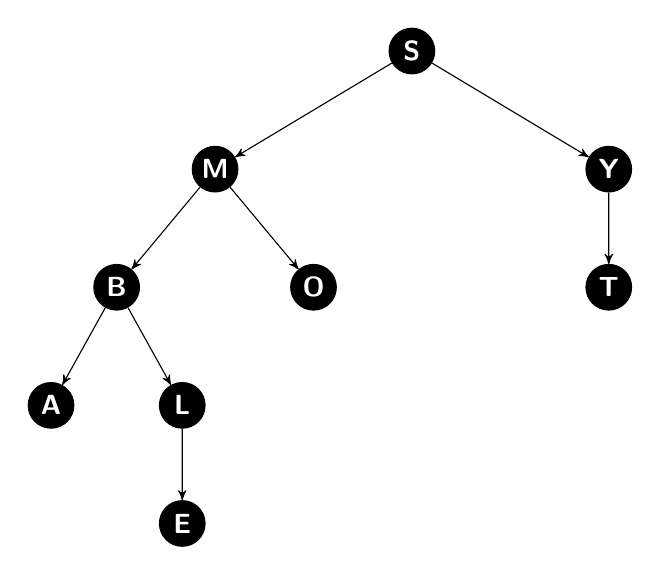
\begin{tikzpicture}[->,>=stealth',level/.style={sibling distance = 5cm/#1,
  level distance = 1.5cm}] 
\node [1] {S}
    child{ node [1] {M} 
            child{ node [1] {B} 
            	child{ node [1] {A} edge from parent node[above left]
                         {}} %for a named pointer
							child{ node [1] {L}
								child{ node[1]{E}}}
            }
            child{ node [1] {O}
            }                            
    }
    child{ node [1] {Y}
            child{ node [1] {T} 
            }
		}
; 
\end{tikzpicture}
\\
Sizes
\\
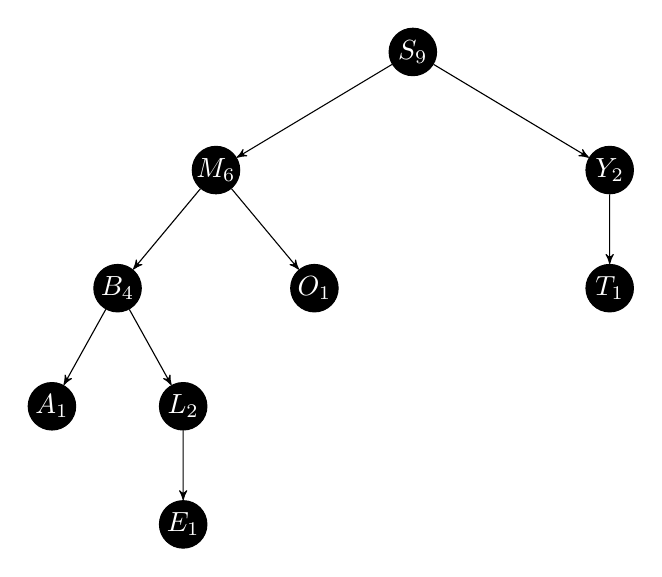
\begin{tikzpicture}[->,>=stealth',level/.style={sibling distance = 5cm/#1,
  level distance = 1.5cm}] 
\node [1] {$S_{9}$}
    child{ node [1] {$M_6$} 
            child{ node [1] {$B_4$} 
            	child{ node [1] {$A_1$} edge from parent node[above left]
                         {}} %for a named pointer
							child{ node [1] {$L_2$}
								child{ node[1]{$E_1$}}}
            }
            child{ node [1] {$O_1$}
            }                            
    }
    child{ node [1] {$Y_2$}
            child{ node [1] {$T_1$} 
            }
		}
; 
\end{tikzpicture}
\\
\newpage
Values[]
\\
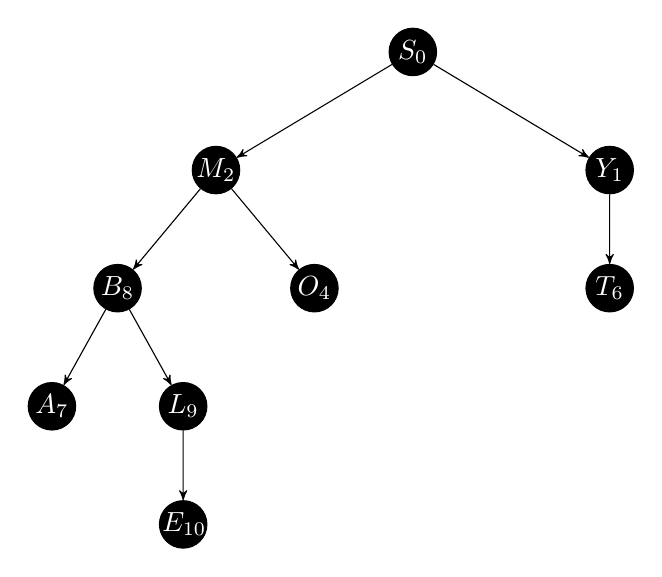
\begin{tikzpicture}[->,>=stealth',level/.style={sibling distance = 5cm/#1,
  level distance = 1.5cm}] 
\node [1] {$S_{0}$}
    child{ node [1] {$M_2$} 
            child{ node [1] {$B_8$} 
            	child{ node [1] {$A_7$} edge from parent node[above left]
                         {}} %for a named pointer
							child{ node [1] {$L_9$}
								child{ node[1]{$E_{10}$}}}
            }
            child{ node [1] {$O_4$}
            }                            
    }
    child{ node [1] {$Y_1$}
            child{ node [1] {$T_6$} 
            }
		}
; 
\end{tikzpicture}
\end{enumerate}

\end{document}